\begin{figure*}[t]
\centering
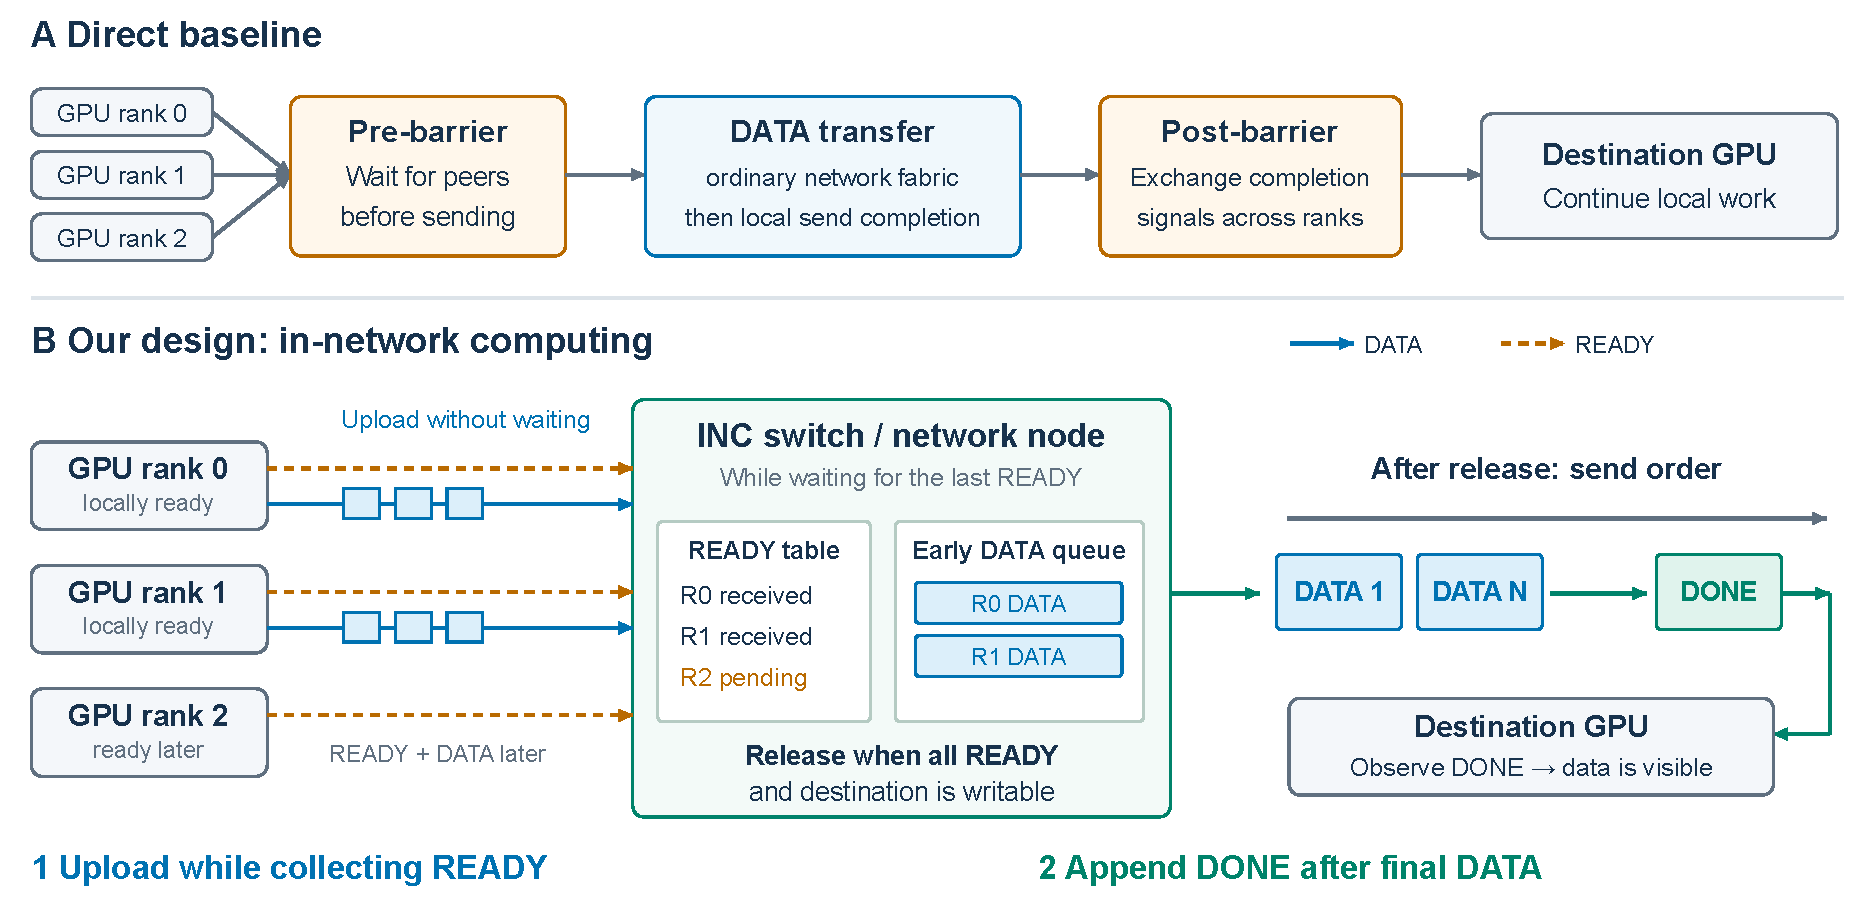
\includegraphics[width=\textwidth]{figures/inc-overview.pdf}
\caption{Two changes to Direct coordination: upload data while collecting READY, then append ordered DONE after the destination's final data. The queue shows the waiting stage; the right-hand sequence shows transmission after forwarding starts. Destination writability, data visibility, and buffer-lifetime requirements remain.}
\Description{The Direct baseline serializes pre-barrier, data transfer and sender completion, and post-barrier. With INC, ranks zero and one upload while rank two is not yet ready. The network stores READY state and early data. Once all ranks are ready, it sends data followed by DONE to the destination.}
\label{fig:design-overview}
\end{figure*}
